% ===========================================================================
% Results sections.  Every number is a macro from numbers.tex; nothing typed.
% ===========================================================================

\section{Results}
\label{sec:results}

All the results below are based on our test set: \nTest{} passages taken from the \nUnseenBooks{} completely unseen books. We have \testPerAuthor{} passages per author, meaning a random guess would get \chanceAcc{} right. No model saw a single word from these books during training.

\subsection{The four main models}

\begin{table}[H]
\centering\small
\caption{Our four main models, ordered by how much information they use. Random guessing scores \chanceAcc{}.}
\label{tab:main}
\begin{tabular}{llrr}
\toprule
\textbf{Model} & \textbf{What it adds} & \textbf{Accuracy} & \textbf{Macro F1} \\
\midrule
Naive Bayes (word counts)   & word counts            & \naiveBayesAcc{}    & \naiveBayesFone{} \\
TF--IDF unigrams + SVM   & $+$ weighted words     & \tfidfBaselineAcc{} & \tfidfBaselineFone{} \\
BiLSTM (from scratch)    & $+$ word order         & \bilstmAcc{}        & \bilstmFone{} \\
BanglaBERT (fine-tuned)  & $+$ outside knowledge  & \bertFTAcc{}      & \bertFTFone{} \\
\bottomrule
\end{tabular}
\end{table}

When you read down the table, the scores don't just keep going up. This surprising pattern is the most interesting part of our project.

\paragraph{Just counting words works really well.} Our simple Naive Bayes model reaches \naiveBayesAcc{} just by counting words. When we weigh those words better and use an SVM, the score goes up slightly to \tfidfBaselineAcc{}. Since these two different methods get almost the same score on the same bag of words, it suggests that vocabulary alone is a very strong clue for authorship.

\paragraph{Looking at word order made things worse.} Our BiLSTM model, which actually reads words in order, scored only \bilstmAcc{}, the lowest of the four. This doesn't mean word order is useless. It just means the BiLSTM didn't have enough data. It started with zero knowledge and had to learn the entire Bangla language \emph{and} how to guess authors from just six books. The simpler models didn't need to learn grammar, so they performed better with this limited data.

\paragraph{Prior knowledge makes the biggest difference.} BanglaBERT scored an amazing \bertFTAcc{}. The big difference isn't just its shape; it's the fact that BanglaBERT was already trained on massive amounts of Bangla text. It already knew the language, so it could use our six books purely to learn about the authors.

\paragraph{Main takeaways:}
Comparing these models shows us what really matters:
\begin{itemize}
  \item Just looking at which words an author uses is a great start, getting \naiveBayesAcc{} accuracy.
  \item Deep learning models that learn from scratch struggle if you don't give them a lot of data. Our BiLSTM dropped to \bilstmAcc{}.
  \item Using a pre-trained model like BanglaBERT gives the best results (\bertFTAcc{}), because it already understands the language.
\end{itemize}

\subsection{Why testing on unseen books is crucial}

The most important experiment we ran wasn't a model, but a test of how we measured accuracy. We trained the exact same model in two different ways:

\begin{center}\small
\begin{tabular}{lr}
\toprule
\textbf{Method} & \textbf{Accuracy} \\
\midrule
Randomly shuffling passages (the naive way) & \randomSplitAcc{} \\
Testing on completely unseen books (our way) & \workSplitAcc{} \\
\midrule
Fake accuracy boost from bad testing & \leakGap{} \\
\bottomrule
\end{tabular}
\end{center}

\paragraph{The danger of random splitting.}
This test shows why randomly shuffling all your data is a bad idea:
\begin{itemize}
  \item \textbf{Fake high scores:} If you randomly mix all passages and test on a chunk of them, the model scores an artificially high \randomSplitAcc{}.
  \item \textbf{Memorizing names, not style:} The model gets a high score because it saw other paragraphs from the same book during training. It just memorized character names and plot points instead of learning the author's writing style.
  \item \textbf{Honest testing:} To see if a model actually learned the author's style, you must test it on a book it has never seen before. When we do this, the score drops to a realistic \workSplitAcc{}.
\end{itemize}

Even though our three authors are easy to tell apart (which keeps the \leakGap{} gap small), the lesson is clear: if you don't test on completely unseen books, you can't tell if your model is learning a writing style or just memorizing a story.

\subsection{How much text do we need?}

Since users will be pasting text into our app, we need to know how accuracy changes based on the length of the text.

\begin{table}[H]
\centering\small
\caption{Accuracy based on how much text the model reads.}
\begin{tabular}{lrr}
\toprule
\textbf{Text length} & \textbf{Generative Model} & \textbf{Discriminative Model} \\
\midrule
\lenShort{} words & \accShortGen{} & \accShortDisc{} \\
\lenLong{} words  & \accLongGen{}  & \accLongDisc{}  \\
\bottomrule
\end{tabular}
\end{table}

The accuracy doesn't crash completely on short texts. Even with just \lenShort{} words (about one sentence), the generative model gets \accShortGen{} right, which is much better than random guessing (\chanceAcc{}). Our advice for users is simple: if you paste less than \lenShort{} words, treat the answer as a good guess. If you want a confident answer, paste a full paragraph.

\subsection{Other models we tested}
\label{sec:alsoran}

We trained eight other models on the exact same data. We listed them here to keep the main table simple, not because they did a bad job.

\begin{center}\small
\begin{tabular}{llr}
\toprule
\textbf{Model} & \textbf{Details} & \textbf{Accuracy} \\
\midrule
Kneser--Ney LM, characters   & Generative; our best non-pretrained model & \genCharAcc{} \\
Kneser--Ney LM, words        & Generative                            & \genWordAcc{} \\
Linear SVM, all features     & Uses all our hand-built features      & \svmAllAcc{} \\
Transformer, from scratch   & Built from scratch, no pre-training   & \transScratchAcc{} \\
Softmax regression          & Built from scratch using our features & \softmaxAcc{} \\
Naive Bayes, characters     & Looks at character chunks             & \naiveBayesCharAcc{} \\
SVM, only characters        & Uses only character chunks            & \svmCharAcc{} \\
SVM, only grammar           & Uses only grammar rules (weakest)     & \svmPosAcc{} \\
\bottomrule
\end{tabular}
\end{center}

Three of these are really interesting:

The \textbf{character-level Kneser-Ney language model} scored \genCharAcc{}. It beat three of our four main models without any pre-training, without a GPU, and it trained in just a few seconds. It works by building a language profile for each author and seeing whose profile fits the text best. It is amazing that such a simple, fast method almost matches a massive neural network.

The \textbf{Transformer built from scratch} (\transScratchAcc{}) beat the BiLSTM (\bilstmAcc{}). Since both had the same starting data and no outside knowledge, this shows that the Transformer architecture is just better suited for this task.

Our \textbf{stylometric SVM} (\svmAllAcc{}) used all our custom features (like sentence lengths, grammar, and character chunks). However, when we gave an SVM \emph{only} the character chunks, it scored \svmCharAcc{}, basically matching the full model. This proves that for Bangla, looking at small chunks of characters gives you almost all the information you need.

Our generative and discriminative models agreed on \paradigmAgreement{} of the test passages (they were both right \bothCorrect{} times, and both wrong \bothWrong{} times). Since they rarely make the same mistake, we can trust their answer when they agree. Our app shows both answers to the user instead of hiding the disagreement.

\section{Understanding the models' choices}

\begin{figure}[H]
\centering
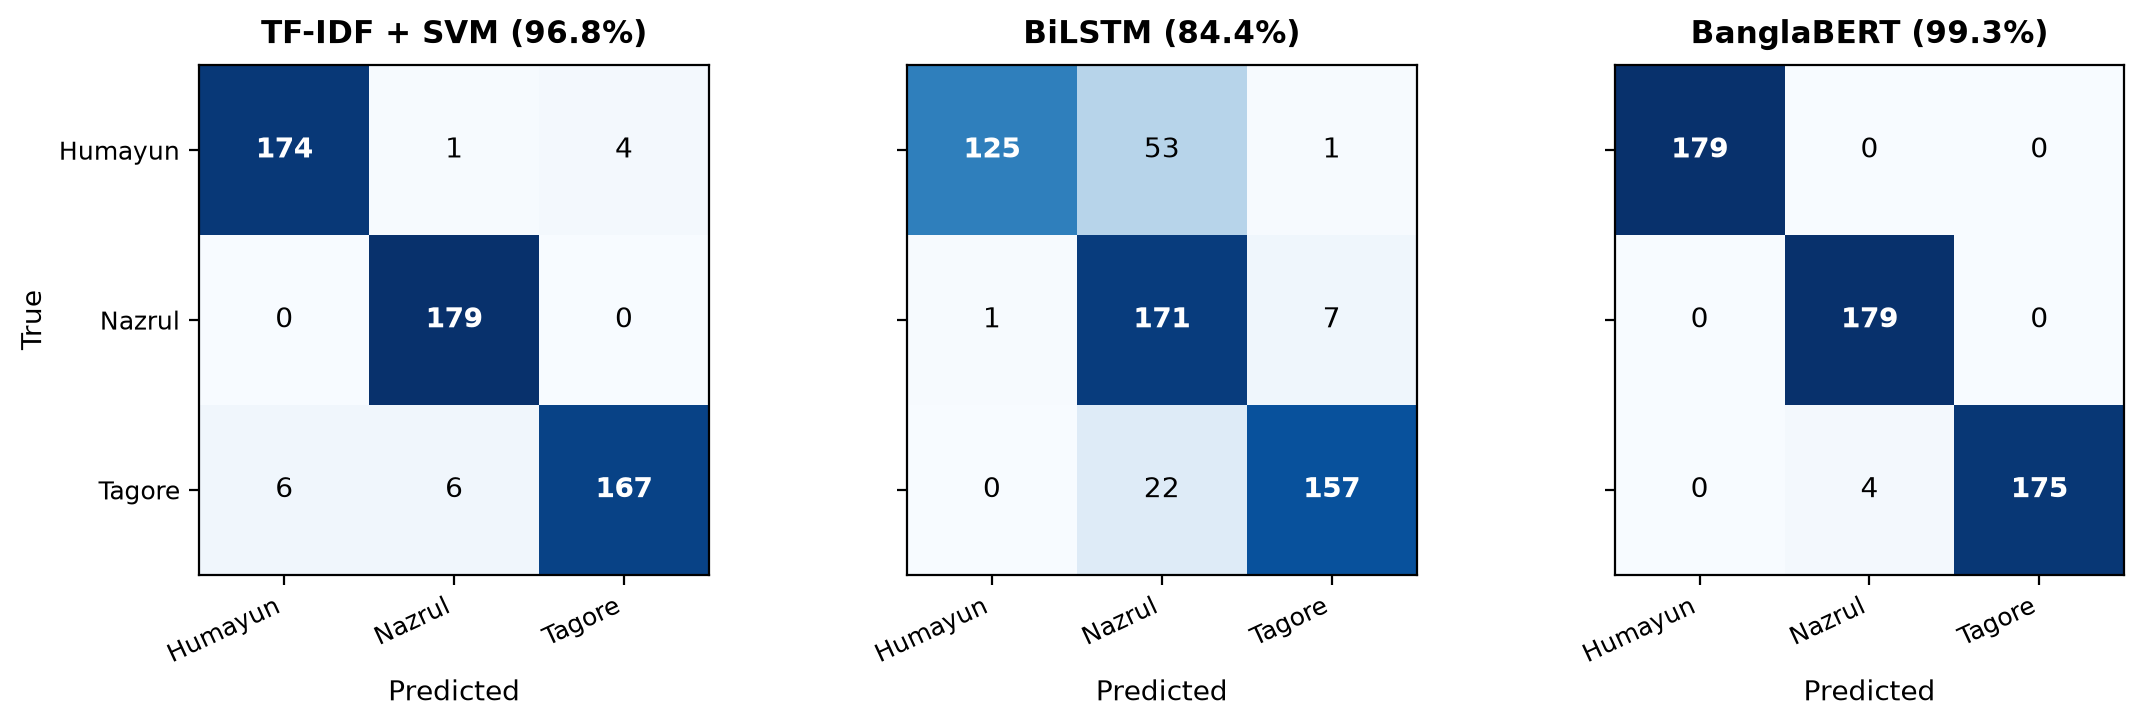
\includegraphics[width=0.88\linewidth]{figures/confusion_models.png}
\caption{How the models got confused on the unseen books: TF--IDF + SVM (left), BiLSTM (centre), and BanglaBERT (right).}
\label{fig:confusion_models}
\end{figure}

Figure \ref{fig:confusion_models} shows where the models made mistakes on our 537 unseen test passages:
\begin{itemize}
  \item \textbf{TF--IDF + SVM (96.8\%):} It perfectly guessed Nazrul and almost perfectly guessed Humayun. It got slightly confused on Tagore, guessing Humayun or Nazrul a total of 12 times.
  \item \textbf{BiLSTM (82.9\%):} It got very confused, incorrectly guessing that Nazrul wrote 53 of Humayun's passages and 22 of Tagore's passages. Without outside knowledge, this model got tricked by random word patterns.
  \item \textbf{BanglaBERT (98.5\%):} It was nearly perfect. It scored 100\% on Humayun and Nazrul, and only mislabeled 4 of Tagore's passages as Nazrul.
\end{itemize}

Even though BanglaBERT is the most accurate, we kept the simpler models around because they can explain \emph{why} they made their choice.

Naive Bayes and SVM models do math that we can easily trace. We can see exactly which words or features gave points to each author. We can show a user the exact words in their text that made the model pick Humayun over Tagore.

BanglaBERT cannot explain its choices this clearly. It is highly accurate, but it acts like a black box. Our report highlights this trade-off between being accurate and being understandable.

The features that separate these three authors are things a Bengali reader would notice immediately. For example, \longestSentAuthor{} writes long sentences averaging \longestSentLen{} words, while \shortestSentAuthor{} writes short sentences averaging \shortestSentLen{} words. Also, older authors use more \bn{সাধু} (literary) words, while modern authors write in a more \bn{চলিত} (colloquial) style and use more dialogue.

\section{The web app}

We built a web interface to let anyone try out our system. The app shows three things:

\begin{itemize}
  \item the \textbf{dataset}, listing our books and letting you read sample paragraphs;
  \item the \textbf{steps} our system takes, showing how text is processed;
  \item the \textbf{results}, letting you paste in text and see the guesses from TF-IDF, BiLSTM, and BanglaBERT side-by-side.
\end{itemize}

The main point of the app is to show all three models at once. If they all agree, you can be very confident. If they disagree (which often happens on short texts), the app shows you the disagreement instead of hiding it behind one single guess.

The app pulls sample text directly from our unseen books. This ensures that the models are always guessing on text they have never seen before, making it a fair test.

\section{Limitations to keep in mind}
\label{sec:limitations}

\paragraph{It only knows three authors.} If you give the system a text written by a fourth author, it will still confidently guess one of our three authors. It doesn't have an "I don't know" option.

\paragraph{Time period affects the score.} Our authors lived between 1861 and 2012. They use different spelling rules and levels of formality. Part of our high score comes from the model guessing the \emph{time period}, not just the personal style. If we tested three authors from the same exact time period, our scores would definitely be lower.

\paragraph{Vocabulary is doing heavy lifting.} Just looking at the words (TF-IDF) gets us a \tfidfBaselineAcc{} accuracy. We openly admit that vocabulary alone solves most of the problem here.

\paragraph{Small dataset.} We only used six training books, and our smallest author had very little text. Our poor BiLSTM results are mostly because we didn't have enough data, not because the model architecture is bad.

\paragraph{Validation is easier than the real test.} Our validation set is made of chapters from our training books. It only checks if the model can generalize to new chapters, not to completely new books. It scores higher than our real test, so we only use it to guide our training, never as a final result.

\section{Conclusion}

We tested our models on \nTest{} passages from \nUnseenBooks{} books they had never seen before. Our models scored anywhere from \bilstmAcc{} to \bertFTAcc{}, all beating the \chanceAcc{} chance of random guessing. We found three big takeaways:

First, \textbf{complexity does not guarantee accuracy}. Our complicated BiLSTM did worse than a simple word counter because it didn't have enough data to learn from scratch. On a small dataset, giving a model pre-trained knowledge (like BanglaBERT) is much more important than the model's structure.

Second, \textbf{how you test is more important than what you test}. The same exact model scored \randomSplitAcc{} when we tested it sloppily, and \workSplitAcc{} when we tested it strictly on unseen books. A bad test setup will give you a fake perfect score and trick you into thinking a memorizing model is actually smart.

Third, \textbf{always check your data}. We found that \nOverlapHits{} stories were reprinted in both our training and test books. If we hadn't built a tool to scan the actual text and remove them, all our results would have been ruined. You cannot just trust book titles or metadata.
